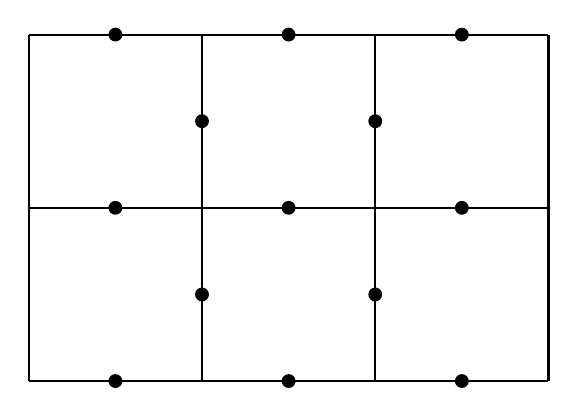
\begin{tikzpicture}[scale=2.2]
   
    \draw[thick] (0,0) grid (3,2);
    
   
    \tikzset{dot/.style={circle, fill=black, inner sep=0pt, minimum size=5pt}}
    
    
    \foreach \x in {0, 1, 2} {
        \foreach \y in {0, 1, 2} {
            \node[dot] at (\x+0.5, \y) {};
        }
    }
    
    \foreach \x in {1, 2} {
        \foreach \y in {0, 1} {
            \node[dot] at (\x, \y+0.5) {};
        }
    }
    
\end{tikzpicture}